%
% !TeX root =./main.tex
% !TeX spellcheck = en_US
\subsection{Matrix Representation of the Road Network}

For now, we consider the \textit{higher level road network} in Carinthia, Austria,
i.e., \textit{A}, \textit{S}, \textit{L}, \textit{B}, in the  form of a matrix.
The vertices of the matrix are the crossing points of the roads, while
the road section connecting those points form the edges of the matrix.
For each edge, we have the distance between the vertices and the length of the bridges along the segment
and the capacity constraints (and the lowest encountered bridge capacity).
This way, we can answer various questions concerning transports between those vertices.
Without loss of generality, we assume an undirected graph.
In that sense, the travel distance along an edge is independent of
the travel direction, and  the same bridges are surpassed in both directions.
The problem statement can
easily be extended to a directed graph. However, the authors omitted this for reasons of simplicity.

Classically,  the considered network consists of
\begin{itemize}
  \item \emph{Nodes} $\mathcal{N}=\{1,\ldots, n\}$, which represent the intersections of different road segments as
  well as the start (end) points of the road segments, and

  \item \emph{Links} $\mathcal{L} \subseteq \mathcal{N} \times \mathcal{N}$,
  representing the road network connecting the road segments.
\end{itemize}

Road links $\ell \in \mathcal{L}$ have a length $d(l)\in \mathbb{R}^{+}$ representing their road length.
Further, they have a weights $c(l) \in C$ giving their \emph{classification} according to {\color{red} ??}.
The classes $C$ describe the level of the roads {\color{red} ??},
while they have an ordering they are an dimensionless quantity.

Bridges (and other types of building structures that must be overpassed)
have \emph{weight limits} (measured in metric tons) which are determined by civil engineers.
Each road link $\ell \in \mathcal{L}$ contains a nonnegative number of bridges, where each has a weight limit.
For each link $\ell$, we set a \emph{weight limit} $w(\ell) \in \mathbb{R}^{+}$ which is the
minimum over all bridges on this link and the \emph{number of bridges} $b(\ell) \in \mathbb{N}^{0}$.
A weight limit $w(\ell)= \infty$ describes the circumstance
that no limit is given for $\ell$.
Similarly, we assume that nodes $n \in \mathcal{N}$ can have weight limits.
\begin{figure}[!ht]
 \centering
  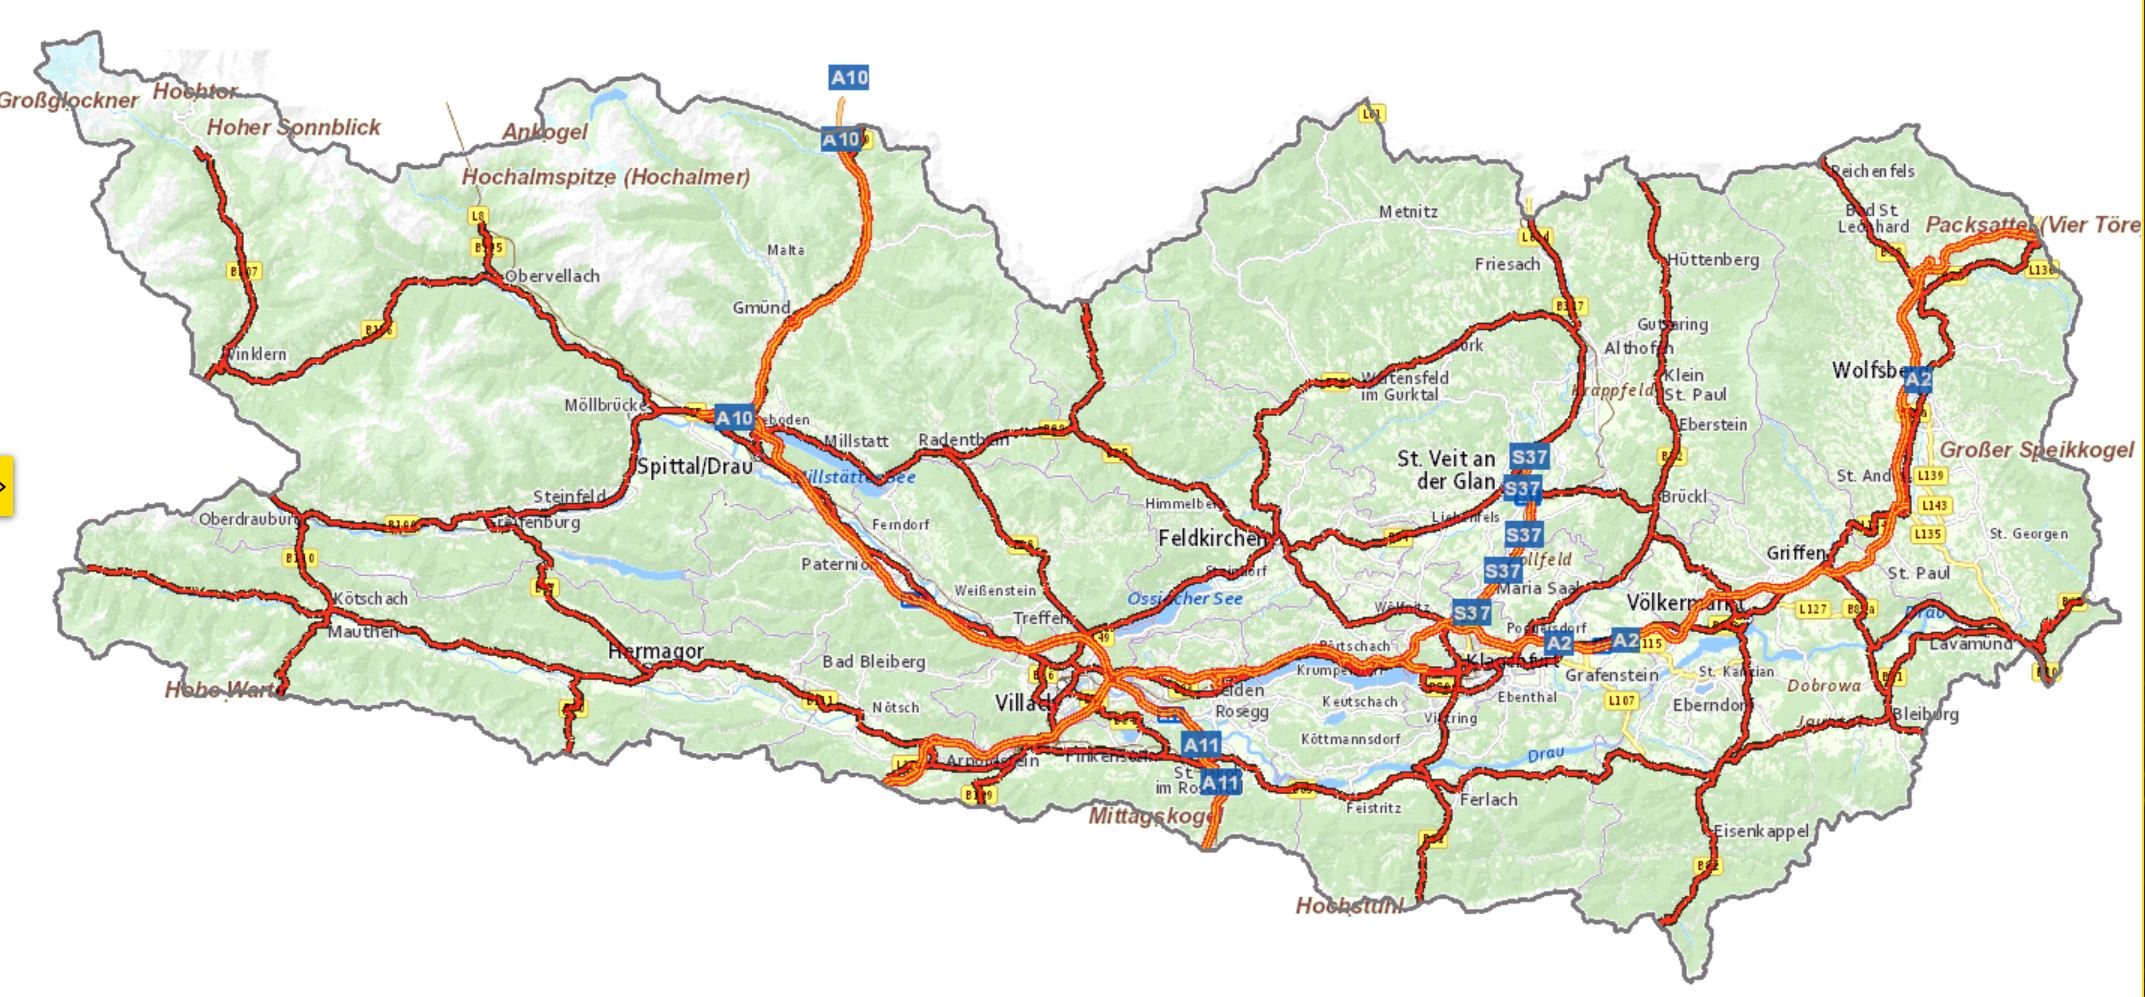
\includegraphics[width=0.9\textwidth]{map.jpg}
  \caption{Overview of the higher level road network in Carinthia.}
  \label{fig:higher level}
\end{figure}


A simple toy example, see Figure \ref{fig_toy_example_1}, shall illustrate these definitions.
\begin{figure}[!ht]
  \centering
  % !TeX root =../main.tex
% !TeX spellcheck = en_US



% https://tex.stackexchange.com/questions/64252/tikz-midway-label-on-a-bended-line
% https://texample.net/tikz/examples/p2p-topology/

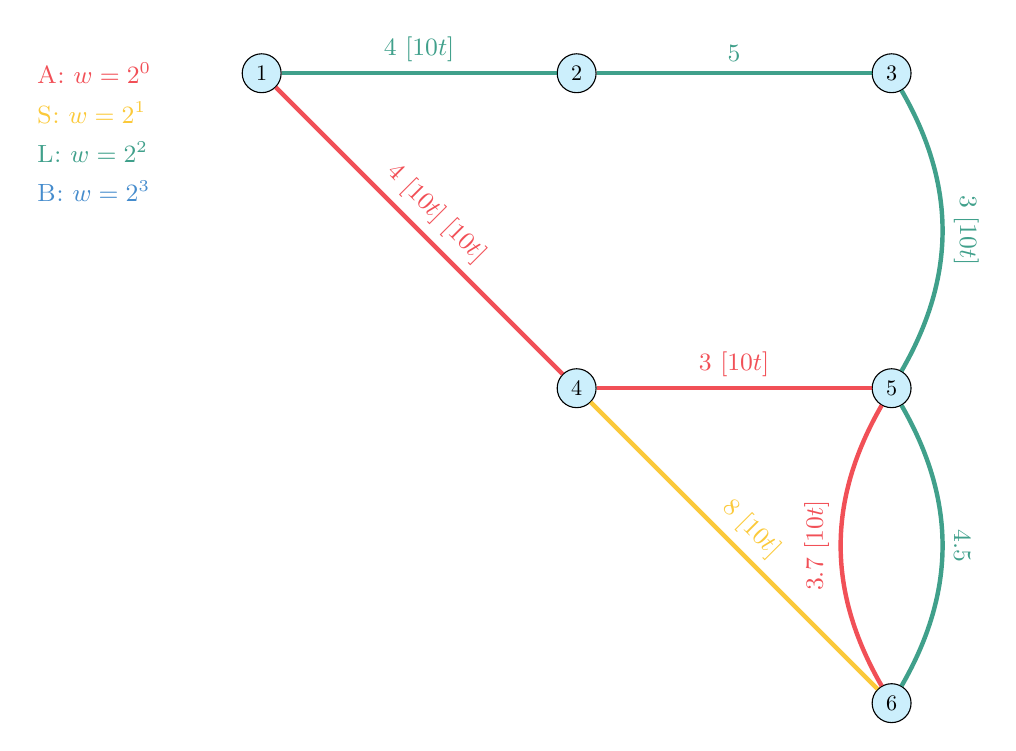
\begin{tikzpicture}[auto, thick]

  % Define Colors
  \definecolor{pinegreen}{cmyk}{0.92,0,0.59,0.25}
  \definecolor{royalblue}{cmyk}{1,0.50,0,0}
  \definecolor{lavander}{cmyk}{0,0.48,0,0}
  \definecolor{violet}{cmyk}{0.79,0.88,0,0}
  \definecolor{red}{cmyk}{0,0.95,0.90,0}
  \definecolor{yellow}{cmyk}{0,0.25,1,0}

  % Node styles
  \tikzstyle{cblue}=[circle, draw, thin,fill=cyan!20, scale=0.8]
  \tikzstyle{qgre}=[rectangle, draw, thin,fill=green!20, scale=0.8]

  \tikzstyle{A_path}=[ultra thick, red, opacity=0.8, font=\small]
  \tikzstyle{S_path}=[ultra thick, yellow, opacity=0.8, font=\small]
  \tikzstyle{B_path}=[ultra thick, royalblue, opacity=0.8, font=\small]
  \tikzstyle{L_path}=[ultra thick, pinegreen, opacity=0.8, font=\small]


  % Nodes
  % \node[cblue] (n_1_1) at (0,0) {1};
  % \node[cblue] (n_2_1) at (4,0) {2};
  \node[cblue] (n_6) at (8,0) {6};

  % \node[cblue] (n_1_2) at (0,4) {4};
  \node[cblue] (n_4) at (4,4) {4};
  \node[cblue] (n_5) at (8,4) {5};

  \node[cblue] (n_1) at (0,8) {1};
  \node[cblue] (n_2) at (4,8) {2};
  \node[cblue] (n_3) at (8,8) {3};




  %  A links

  \draw[A_path] (n_4)--  (n_5)  node [midway, above, sloped] (TextNode) {$3~[10t]$};
  \draw[A_path] (n_6) to[bend left]   node [midway, above, sloped]  {$3.7~ [10t]$} (n_5)  ;
  \draw[A_path] (n_4) -- (n_1)  node [midway, above, sloped] (TextNode) {$4 ~[10t]~[10t]$};


  % S links
  \draw[S_path] (n_4) to node [midway, above, sloped] {$8~ [10t]$} (n_6);

  %  L lines
  \draw[L_path] (n_1) --  (n_2)  node [midway, above, sloped] (TextNode) {$4~[10t]$};

  \draw[L_path] (n_2)--  (n_3)  node [midway, above, sloped] (TextNode) {$5$};
  % \draw[L_path] (n_3) to[out=-20,in=-20]  (n_5)  node [midway, above, sloped] (TextNode) {$l=3, b=2$};
  \draw[L_path] (n_3) to[bend left] node [midway, above, sloped]   {$3~[10t]$}    (n_5);


  \draw[L_path] (n_5) to[bend left]  node [midway, above, sloped] {$4.5$} (n_6);

  % B links
  % \draw[B_path] (n_6) to node [midway, above, sloped] {$7; 2$} (n_2_1);


  % Legends
  \node[A_path, anchor=west] at (-3,8){\textsc{A:} $w=2^0$};
  \node[S_path,anchor=west] at (-3, 7.5){\textsc{S:} $w=2^1$};
  \node[L_path,anchor=west] at (-3, 7){\textsc{L:} $w=2^2$};
  \node[B_path,anchor=west] at (-3, 6.5){\textsc{B:} $w=2^3$};

\end{tikzpicture}

  \caption{Toy Example 1.}
  \label{fig_toy_example_1}
\end{figure}


\subsection{Related Work on the Shortest Path Problem}

\citet{TACCARI2016122}

\subsection{Mathematical Model}


\begin{align*}
   \min \sum    \\
   \text{s.t.}  &  \\
    & \sum
\end{align*}
